\documentclass[italian,12pt,a4paper,oneside,final]{report}
\usepackage[toc]{appendix}
\usepackage{listings}
\usepackage{graphicx}
\usepackage{biblatex} %Imports biblatex package
\usepackage[utf8]{inputenc}
\usepackage[italian]{babel}
\usepackage{csquotes}
\usepackage{hyperref}
\addbibresource{iot.bib} %Import the bibliography file
\graphicspath{ {images/} }
\lstset{captionpos=b,showspaces=false,basicstyle=\ttfamily,showstringspaces=false,breaklines=true}
\renewcommand{\thesection}{\arabic{section}} % remove the \chapter counter from being printed with every \section
\renewcommand{\appendixtocname}{Appendice}
\renewcommand{\appendixpagename}{Appendice}
\hypersetup{
	colorlinks=true,
	linkcolor=,
	pdftitle={Marco Giunta - Progetto IoT},
	pdfauthor={Marco Giunta},
}

\title{\huge Power Meter Wi-Fi con Arduino\\[0.5em]
\large Relazione Progetto IoT}
\date{Ottobre 2022}
\author{
Marco Giunta\thanks{Marco Giunta 147852 giunta.marco@spes.uniud.it}}

\begin{document}
% Generate title page
\maketitle

% Generate TOCs
\pagenumbering{arabic}
\tableofcontents

\newpage

\section{Introduzione}
Una delle sfide chiave del XXI secolo è l’adattamento ai cambiamenti climatici.
Per riuscire a limitare il riscaldamento globale, è necessario impiegare l’energia in modo efficiente, riducendo il consumo all'interno delle proprie abitazioni o negli edifici pubblici.
Per decidere quali misure adottare, è indispensabile conoscere il consumo reale delle apparecchiature che usiamo ogni giorno.

Con questo progetto si vuole realizzare un prototipo a basso costo di un misuratore di consumo elettrico collegato ad una rete locale tramite \mbox{Wi-Fi}.
Il progetto ha come obiettivo l’acquisizione e il monitoraggio dei valori di tensione, corrente e potenza presenti ai capi di un qualunque apparecchio collegato alla rete elettrica domestica (220V).
Il codice presente all'interno del dispositivo è stato progettato per permettere il collegamento contemporaneo di circa 65.000 unità, in modo da poter monitorare, ad esempio, tutte le apparecchiature presenti all'interno di un istituto di ricerca.

Per garantire il monitoraggio di un numero così elevato di dispositivi, è stato necessario ricorrere all'utilizzo del protocollo MQTT\footfullcite{mqtt}, per ottimizzare la gestione della banda di rete e garantire l'autenticazione dei singoli dispositivi.
Per raccogliere i dati è stato utilizzato il sistema di gestione di database InfluxDB\footfullcite{influxdb} mentre, per la parte di visualizzazione tramite dashboard, è stato utilizzato il software Grafana\footfullcite{grafana}.

Per l'installazione e configurazione del broker Mosquitto\footfullcite{mosquitto}, il collettore Telegraf\footfullcite{telegraf}, il database InfluxDB e il software Grafana è stata utilizzata la tecnologia dei container.

\newpage

\section{Componenti}
Per la realizzazione del prototipo sono stati utilizzati questi componenti:

\begin{itemize}
\item Arduino MKR 1000 WiFi
\item Display LCD 16×2
\item Modulo LCM1602 IIC per display LCD
\item Sensore di corrente AC-CC da 5A con ACS712
\item Sensore di tensione con ZMPT101B
\item Divisori di tensione (da 5V a 3.3V)
\end{itemize}


\subsection{Schema elettrico}
\begin{figure}[h]
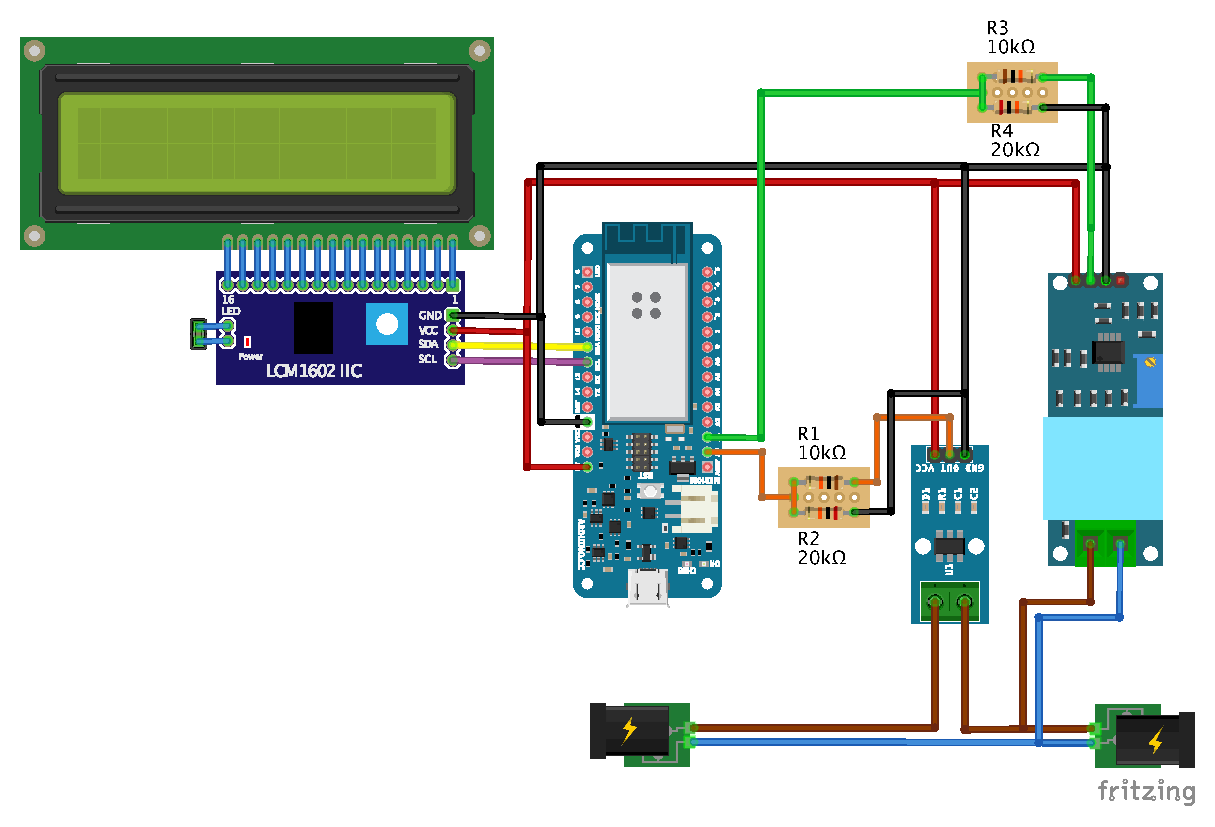
\includegraphics[width=\textwidth]{power_meter_bb.pdf}
\centering
\end{figure}

\subsection{Arduino MKR 1000 WiFi}
La scheda Arduino MKR 1000 WiFi è un prodotto specifico per IoT.
Integra al suo interno un processore Arm Cortex-M0 32-bit SAMD21, un chip di sicurezza ATECC508A e un controller Wi-Fi ATWINC1500.
Ci sono 7 pin d'ingresso analogico (A0-A6) in grado di rilevare una tensione d'ingresso compresa da 0 e 3.3V .

\subsection{Sensore di corrente}
Il sensore di corrente è un modulo che utilizza il sensore ACS712 in grado di misurare correnti fino a 5A.
Quando nessuna corrente attraversa il sensore ACS712, il modulo ha una tensione d'uscita pari a metà della tensione di alimentazione, che deve essere 5V.

Nel modello usato in questo progetto, la tensione di uscita varia di 185 mV per ogni A di corrente rilevata dal sensore.

\subsection{Sensore di tensione}
Il sensore di tensione è un modulo che utilizza il trasformatore ZMPT101B ed è in grado di misurare tensioni fino a 250V AC.
Sulla scheda è presente un potenziometro multigiro per regolare il guadagno dell'uscita ADC.

Quando non è presente nessuna tensione all'ingresso del trasformatore, il modulo ha una tensione d'uscita pari a metà della tensione di alimentazione che, anche in questo caso, deve essere 5V.

\subsection{Display LCD}
Per visualizzare i valori di tensione e corrente misurati dai sensori e quelli di potenza (reale ed apparente) calcolati, è stato utilizzato un display LCD da 16 caratteri a 2 righe.
Il display è pilotato da un modulo LM1602, basato sul chip PCF8574, che permette la connessione di qualunque scheda Arduino attraverso il bus $I^2C$.
Anche questo modulo deve essere alimentato a 5V.

\newpage

\subsection{Divisori di tensione}
I pin d'ingresso analogico della scheda Arduino MKR 1000 WiFi sono in grado di rilevare tensioni fino a 3.3V, mentre i sensori di corrente e tensione funzionano con una tensione di alimentazione di 5V.
Entrambi i sensori hanno una tensione di uscita che varia da 0 a 5V, incompatibile con i pin della scheda Arduino.
Per ovviare al problema sono stati realizzati dei divisori di tensione (figura~\ref{fig:voltage_divider}) in modo da \textit{convertire} il range della tensione di uscita dei sensori da 0-5V a 0-3.3V.

\begin{figure}[h]
	\centering
	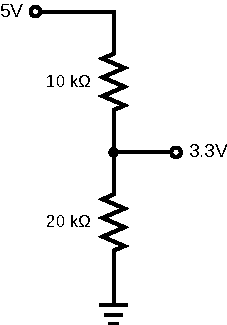
\includegraphics[width=0.25\textwidth]{voltage_divider.pdf}
	\caption{Divisore di tensione}
	\label{fig:voltage_divider}
\end{figure}

\section{Codice Arduino}
Nella fase di \textit{setup}, vengono letti i valori di calibrazione dei sensori (maggiori dettagli nella sezione \ref{section:calibrazione}), connessa la scheda alla rete Wi-Fi e attivato il display LCD.

Prima di attivare la connessione con il broker MQTT, viene generato il \textit{clientID} a partire da un prefisso (\emph{pwrmtr}) e dal valore del terzo e quarto ottetto dell'indirizzo IP.
Se necessario, vengono aggiunti degli zeri ai valori degli ottetti, in modo da ottenere un \textit{clientID} di lunghezza fissa.
In questo modo è possibile collegare circa 65.000 unità senza modificare il codice sorgente.
Per evitare connessioni al broker da parte di client non autorizzati, la connessione è autenticata tramite \textit{username} e \textit{password}.

Nella fase di \textit{loop}, sul display viene visualizzato il valore di corrente e tensione calcolato su una media di 1000 campioni.
Dato che le grandezze misurate dai sensori sono corrente e tensione alternata, per ottenere una misura accurata è stato necessario calcolarne il \emph{valore efficace} (semplificando, il valore equivalente in corrente continua).
Ogni milli secondo viene registrato un campione e ogni mille campioni (ogni secondo) viene calcolato il valore RMS dei campioni in questo modo:
\begin{itemize}
  \item si eleva al quadrato ogni campione, in modo da perdere il segno dei valori negativi
  \item si calcola la media dei quadrati dei campioni
  \item si estrae la radice quadrata della media
\end{itemize}

\noindent Per effettuare queste operazioni è stata usata la libreria Statistical\footfullcite{statistical}.

Sul display sono visualizzati anche i valori di potenza, calcolati su una media di 1000 campioni.
Per ottenere il valore di potenza reale viene fatta la media dei prodotti del valore istantaneo di corrente e tensione dei campioni.
L'unità di misura di questo valore è il Watt.
Mentre per ottenere il valore di potenza apparente viene fatta la media dei prodotti del valore efficace (RMS) di corrente e tensione calcolati in precedenza.
In questo caso l'unità di misura è il Volt Ampere(VA).

Una volta ottenuti tutti i valori, questi vengono inviati al broker MQTT usando un \emph{topic} diverso per ogni valore:

\begin{enumerate}
  \item[]sensors/\textit{clientId}/voltage
  \item[] sensors/\textit{clientId}/current
  \item[] power/\textit{clientId}/real
  \item[] power/\textit{clientId}/apparent
\end{enumerate}

\newpage

\subsection{Calibrazione}\label{section:calibrazione}
La tensione di uscita dei moduli varia tra 0 to 5V in base alla tensione o alla corrente presente all'ingresso: questo valore viene convertito dalla scheda Arduino in un numero compreso tra 0 e 1023.
Come detto in precedenza, quando non è presente nessuna tensione o non c'è assorbimento di corrente, la tensione presente all'uscita dei moduli è pari a metà della tensione di alimentazione degli stessi: visto che i moduli sono alimentati a 5V, la tensione di uscita è circa 2.5V.

A causa delle tolleranze dei componenti presenti all'interno moduli è possibile che ci siano delle fluttuazioni della tensione di uscita.
Per limitare questo problema viene effettuata, in modo automatico, una calibrazione dei sensori al primo avvio dopo la scrittura del codice.
Vediamo più in dettaglio questa procedura.

La prima volta che si accende la scheda dopo aver caricato il codice, non bisogna collegare nulla né all'ingresso né all'uscita del Power Meter: tensione e corrente misurate devono essere pari a zero.

Vengono letti 2000 campioni, calcolata la media dei valori assoluti e definito un valore di \textit{offset} da aggiungere a tutte le successive letture.
Con lo stesso metodo viene calcolata la media dei valori RMS e definito un secondo valore di \textit{offset} da aggiungere a tutti i valori RMS calcolati.
Usando 5000 campioni, viene definito con la stesso tipo di procedura l'ultimo valore di \textit{offset} da aggiungere al calcolo della potenza reale.

Visto che la calibrazione può esser fatta solo quando tensione e corrente misurate sono pari a zero, non è possibile eseguire la procedura ad ogni avvio.
Bisogna salvare i valori degli \textit{offset} all'interno della memoria della scheda Arduino e leggerli ad ogni avvio: purtroppo questo modello non ha una \mbox{EEPROM on-board}.
Fortunatamente nel chip di sicurezza Microchip ATECC508A è presente una EEPROM da 10Kb, spazio più che sufficiente per salvare questi dati.
La EEPROM è in divisa in 16 slot di diversa capacità: secondo quanto indicato sul datasheet, lo slot 8 è il candidato ideale per salvare questo tipo di informazioni visto che la capacità dello slot è di 416 Bytes e i dati da salvare sono in formato \textit{float} (su Arduino occupano 4 Byte\footfullcite{float}).
Anche se per salvare gli \textit{offset} sarebbe sufficiente un blocco da 20 Byte \mbox{(5 offset * 4Byte)}, per eseguire un unica operazioni di lettura/scrittura, si utilizza un blocco di 32 Bytes, dove i restanti sono 12 Byte non sono utilizzati.

\noindent Per effettuare queste operazioni è stata usata la libreria ArduinoECCX08\footfullcite{eccx08}.

La calibrazione viene eseguita solo al primo avvio, per forzare una ricalibrazione basta collegare per un instante il pin 6 al pin GND.
Durante la calibrazione non vengono inviati dati al broker MQTT e sul display appare la scritta in figura~\ref{fig:calibration_in_progress}.

\begin{figure}[h]
	\centering
	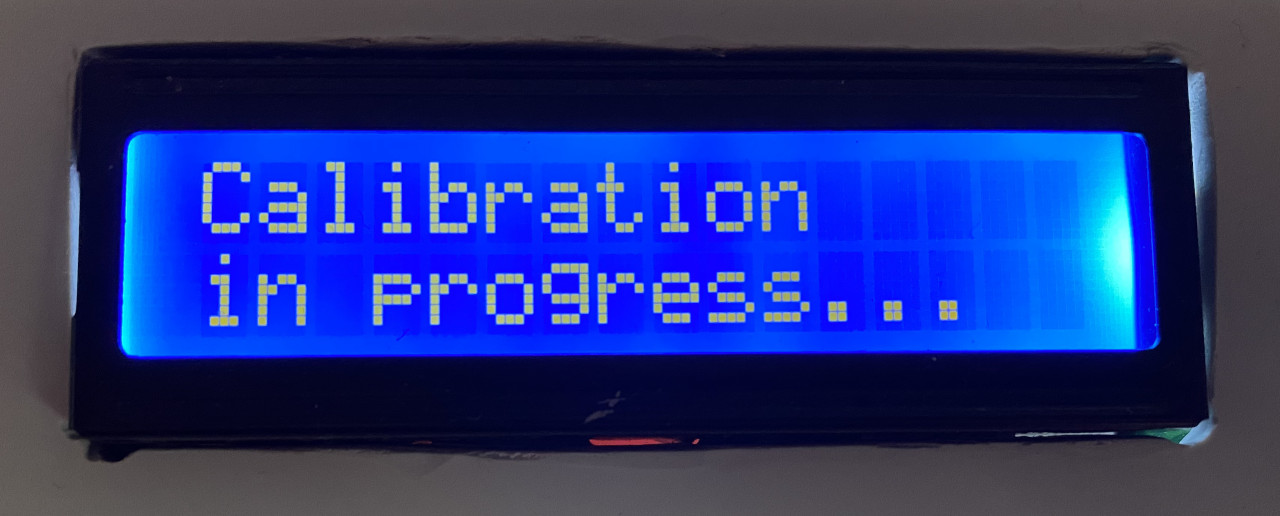
\includegraphics[width=0.75\textwidth]{calibration_in_progress.jpg}
	\caption{Calibrazione in corso}
	\label{fig:calibration_in_progress}
\end{figure}

Dopo avere effettuato la calibrazione automatica, bisogna calibrare il guadagno dell'uscita del sensore di tensione.
Per farlo, bisogna collegare l'ingresso del Power Meter alla rete elettrica, un multimetro in grado di effettuare una misurazione valore RMS di tensione all'uscita e ruotare in senso orario o antiorario il potenziometro multigiro presente sul sensore fino a quando i valori misurati non coincidono (figura~\ref{fig:voltage_calibration}).

\begin{figure}[h]
	\centering
	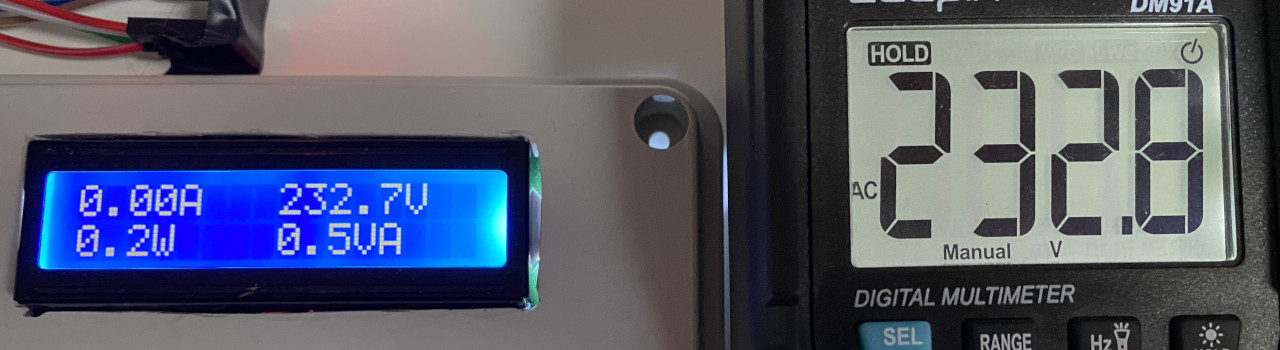
\includegraphics[width=0.75\textwidth]{voltage_calibration.jpg}
	\caption{Calibrazione sensore di tensione}
	\label{fig:voltage_calibration}
\end{figure}

Per evitare problemi nella lettura dei valori quando la tensione misurata è vicina al limite dei 250V AC, il guadagno dell'uscita del sensore è stato ridotto di circa 1/3 all'interno del codice Arduino (\textit{outputGain}).

\section{Presentazione dei dati}
Per visualizzare i dati misurati dal Power Meter è stata realizzata una dashboard Grafana.
Il Power Meter invia i valori rilevati dai sensori ad un broker Mosquitto, i quali vengono presi da un collettore Telegraf e salvati all'interno di un database InfluxDB.
Tutti questi componenti software sono stati installati e configurati usando Docker.

\begin{figure}[h]
	\centering
	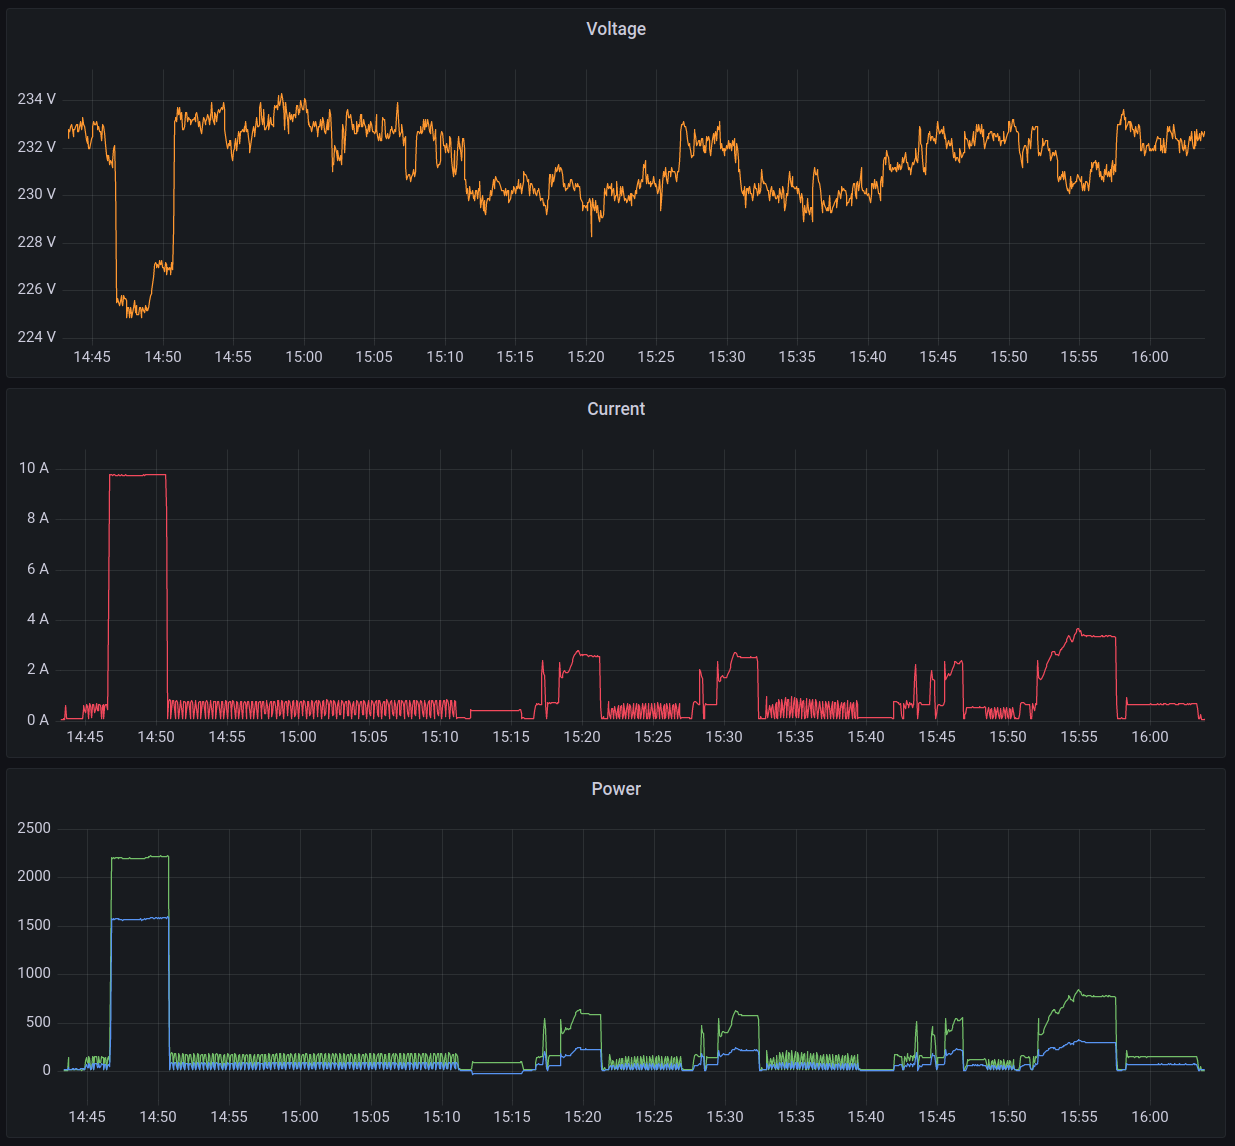
\includegraphics[width=1\textwidth]{grafana_lavatrice.png}
	\caption{Valori rilevati durante un ciclo di lavaggio a $30^\circ C$}
	\label{fig:grafana_lavatrice}
\end{figure}

Nella figura~\ref{fig:grafana_lavatrice} si possono vedere i dati rilevati ai capi di una lavatrice durante un ciclo di lavaggio a $30^\circ C$.
Nella sezione \textit{Power} vengono visualizzati i dati della potenza reale e di quella apparente.


\section{Conclusioni}
Il prototipo realizzato ha raggiunto gli obiettivi previsti: è un misuratore di consumo elettrico, realizzabile a basso costo ed è in grado di inviare i dati tramite la rete Wi-Fi.
Anche se i sensori utilizzati nel progetto non sono di tipo professionale, i valori rilevati sono abbastanza precisi e permettono una valutazione dei consumi reali di un qualunque apparecchio collegato alla rete elettrica.

Data la semplicità e il basso costo di realizzazione, il progetto può essere utilizzato per monitorare i consumi degli apparecchi presenti all'interno di un intero edificio.
Inoltre, la possibilità di visualizzare i consumi in tempo reale, tramite una dash board Grafana, è un aiuto importante nella valutazione di azioni da intraprendere per ridurre i consumi energetici, identificando le apparecchiature più \textit{energivore} o le ore della giornata dove si registrano i consumi più elevati.

\appendices
\noindent{\huge\bfseries APPENDICE\par}

\section{Prototipo}

\begin{figure}[ht]
	\makebox[\textwidth][c]
	{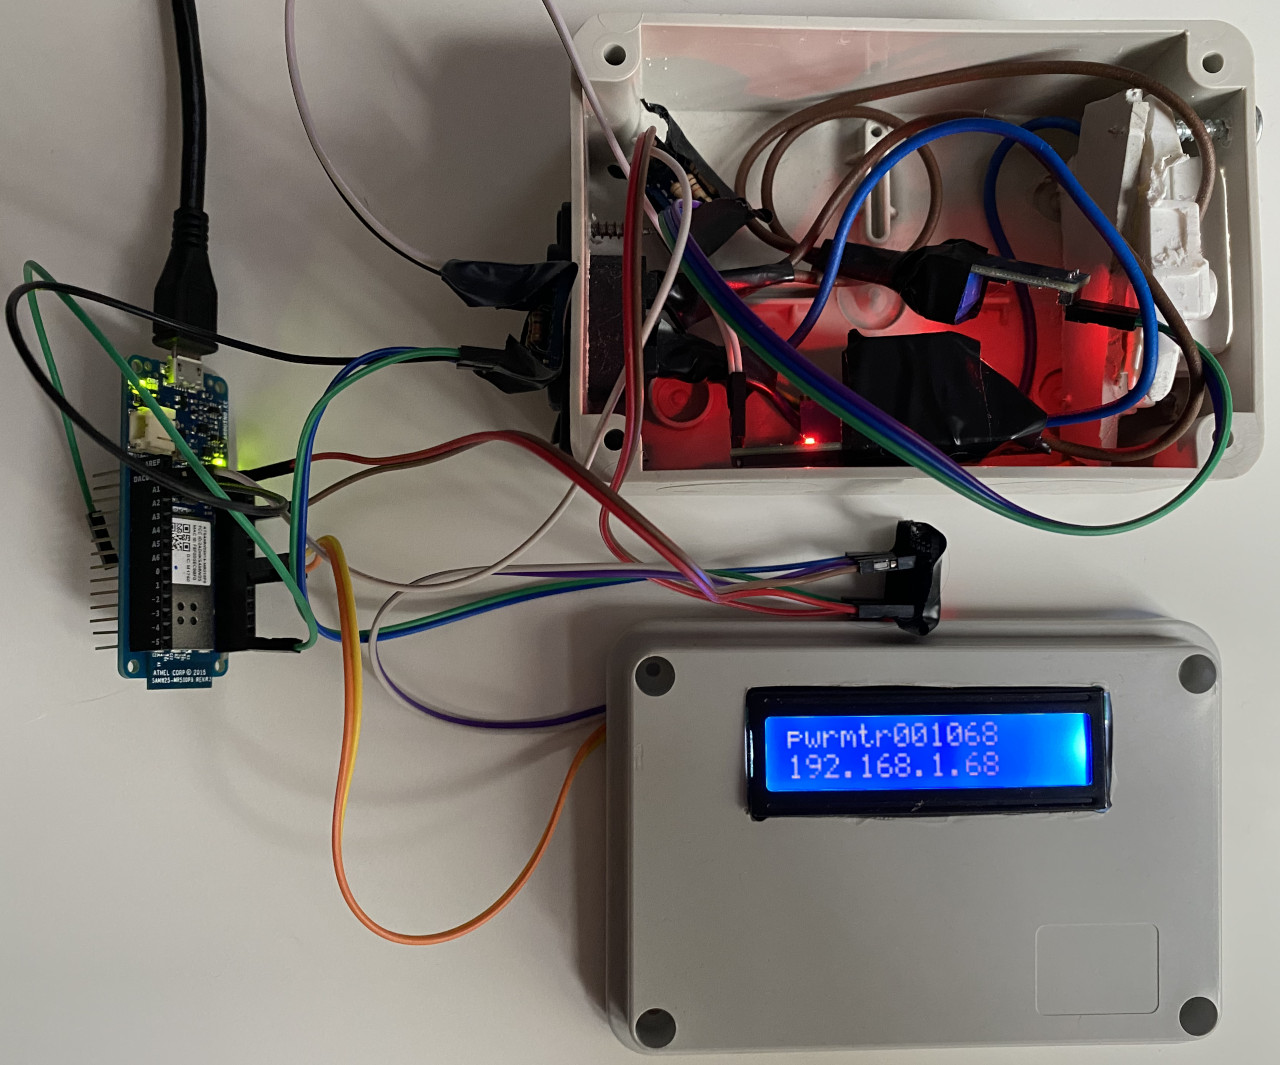
\includegraphics[width=1.3\textwidth]{power_meter_picture.jpg}}
	\caption{Foto del prototipo}
	\label{fig:prototipo}
\end{figure}

\newpage

\section{Docker Compose}
\begin{lstlisting}[caption=docker-compose.yaml]
version: "3.8"
  services:
    influxdb:
      image: influxdb
      environment:
        - TZ=Europe/Rome
        - DOCKER_INFLUXDB_INIT_MODE=setup
        - DOCKER_INFLUXDB_INIT_USERNAME=user
        - DOCKER_INFLUXDB_INIT_PASSWORD=password
        - DOCKER_INFLUXDB_INIT_ORG=org
        - DOCKER_INFLUXDB_INIT_BUCKET=telegraf
        - DOCKER_INFLUXDB_INIT_ADMIN_TOKEN='jcTCQ5PRSjOtj5ur0TkGc9y93aRYb...AdSzVdZu2qCUsV5iaIwQg=='
      ports:
        - "8086:8086"
      networks:
        - iot
      volumes:
        - influxdb/data:/var/lib/influxdb2
        - influxdb/config:/etc/influxdb2
      restart: always

    telegraf:
      image: telegraf
      user: "telegraf"
      environment:
        - TZ=Europe/Rome
      ports:
        - "8125:8125/udp"
      networks:
        - iot
      volumes:
        - telegraf/telegraf.conf:/etc/telegraf/telegraf.conf:ro
      depends_on:
        - influxdb
        - mosquitto
      restart: always

    grafana:
      image: grafana/grafana-oss
      ports:
        - "3000:3000"
      networks:
        - iot
      volumes:
        - grafana/data:/var/lib/grafana
      depends_on:
        - influxdb
      restart: always

    mosquitto:
      image: eclipse-mosquitto
      ports:
        - "1883:1883"
      networks:
        - iot
      volumes:
        - mosquitto/:/mosquitto/
      restart: always

  networks:
    iot:
\end{lstlisting}
	
\section{Configurazione Mosquitto}
\begin{lstlisting}[caption=mosquitto.conf]
allow_anonymous false
password_file /mosquitto/config/password_file
listener 1883
persistence true
persistence_location /mosquitto/data/
\end{lstlisting}

\begin{lstlisting}[caption=password\_file]
telegraf:$7$101$lJSpen5vJKMmX3vj$j5f...dSc9Fs6X1nUeJqjc47AA==
\end{lstlisting}

\section{Configurazione Telegraf}
\begin{lstlisting}[caption=telegraf.conf]
[[inputs.mqtt_consumer]]
servers = ["tcp://mosquitto:1883"]

topics = [
"sensors/#",
"power/#",
]

username = "telegraf"
password = "metricsmetricsmetricsmetrics"

data_format = "value"
data_type = "float"

[[outputs.influxdb_v2]]
urls = ["http://influxdb:8086"]
token = "jcTCQ5PRSjOtj5ur0TkGc9y93aRYb...AdSzVdZu2qCUsV5iaIwQg=="
organization = "org"  
bucket = "telegraf"
\end{lstlisting}

\end{document}
